\begin{que}
	Read about the following plots:
	\begin{enumerate}
		\item Violin Plot
		\item Pareto Chart
		\item Coxcomb Chart
		\item Waterfall Plot
	\end{enumerate}
	Describe the uses of these plots. Take some sample data and generate one example plot
	for each of them.

	\hspace*{\fill} [8 marks]
\end{que}

\begin{tcolorbox}[breakable]
	\begin{sol}
		Here are the descriptions and usages of the given plots along with their examples:
		\begin{enumerate}
			\item \textbf{Violin plot:} It's a hybrid of box plot and kernel density plot.
			      A box plot represents data in a linear fashion. It's made of a straight line
			      from lowest value to highest value along with a box from first to third
			      quartiles, marking all the quartiles of the dataset. Here's an example:
			      \begin{figure}[H]
				      \centering
				      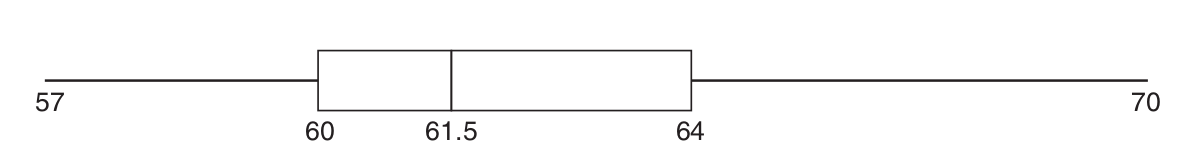
\includegraphics[width=0.5\textwidth]{box_plot}
				      \caption{Box plot}
				      \label{fig:box}
			      \end{figure}
			      A kernel density plot represents the density/frequency of data points. It's
			      similar to a histogram, but smooth. In a violin graph, this is kept vertical,
			      with two mirror images of it reflected along y-axis. This is useful in the
			      sense that we can look into both centrel tendencies of the data (like mean,
			      median etc.) but also how the data is distributed. Both at once. We can
			      visualise the following data which I've taking from (*) containing the average
			      number of hours a person studies given the number of courses taken
			      \begin{figure}[H]
				      \centering
				      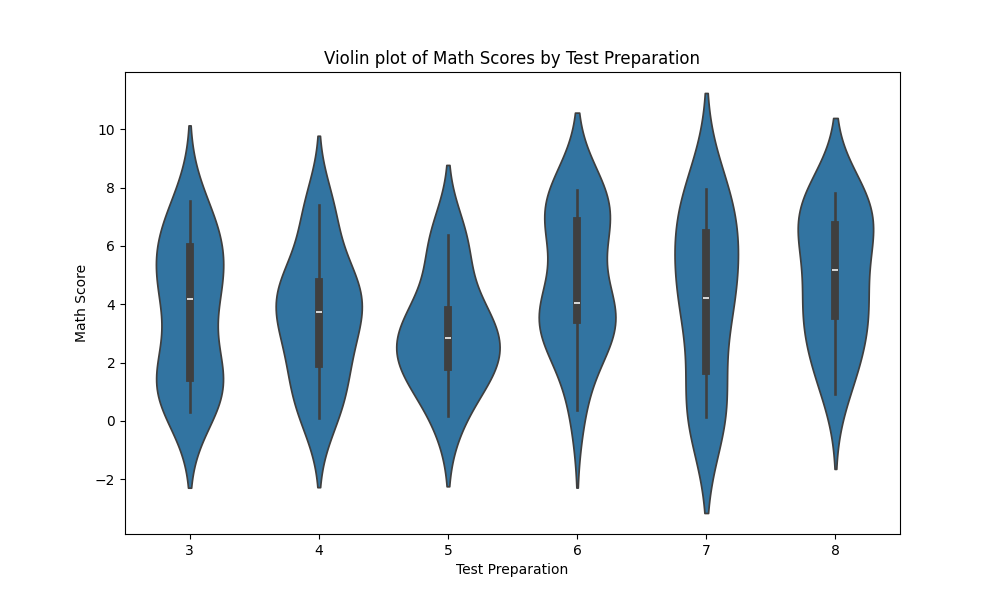
\includegraphics[width=0.7\textwidth]{violin-plot}
				      \caption{Violin Plot}
				      \label{fig:violin}
			      \end{figure}
			      As mentioned before, a violing plot can show both statistical summary along
			      with distribution, which a normal plot can't. Here, the gray line represents
			      the box plot component of it. And the plot you get by rotating it by $90^\circ$
			      is the distribution plot.
			\item \textbf{Pareto Chart:}
		\end{enumerate}
	\end{sol}
\end{tcolorbox}
